\subsection{Additional pipeline details}
\label{subsection:additional_pipeline_details}

\subsubsection{Model training}
\label{subsubsection:model_training_details}

\begin{algorithm}[bh]
\caption{Model training procedure}
\label{algorithm:sded_model_training}
\begin{algorithmic}[1]
\State \textbf{Data definitions:}
\State \quad Input neural data: $\mathbf{Y} \in \mathbb{R}^{B \times S \times N_{\text{in}}}$ \textsuperscript{(Batch, Sequence length, Input neural units)}
\State \quad Target neural data: $\mathbf{Z} \in \mathbb{R}^{B \times \times N_{\text{out}}}$ \textsuperscript{(Batch, Output neural units)}
\State \textbf{Model definitions:}
\State \quad Encoder: $\mathbf{W}_{\text{enc}} \in \mathbb{R}^{D_{\text{max}} \times S \times N_{\text{in}}}$, $\mathbf{b}_{\text{enc}} \in \mathbb{R}^{D_{\text{max}}}$ \textsuperscript{(Hidden layer neurons)}
\State \quad Decoder: $\mathbf{W}_{\text{dec}} \in \mathbb{R}^{N_{\text{out}} \times D_{\text{max}}}$, $\mathbf{b}_{\text{dec}} \in \mathbb{R}^{N_{\text{out}}}$
\State \quad Transformer block (optional) $\mathbf{\theta_{t}}$: $\{\mathbf{W}_{Q,K,V} \in \mathbb{R}^{D_{\max} \times D_{\max}}, \dots\}$
\State \quad Matryoshka levels: $\mathbf{\{D_l\}_{l=1}^L}$
\State \quad Weights each level's reconstruction loss (optional): $\mathbf{\{\lambda_l\}_{l=1}^L}$
\State \quad Auxiliary loss weight: $\mathbf{\gamma}$
\\
\Procedure{train\_step}{$\mathbf{Y}, \mathbf{Z}$}    
    \Statex \Comment{\textit{--- Forward Pass ---}}
    \State $\mathbf{A} \gets \text{ReLU}(\mathbf{Y}\mathbf{W}_{\text{enc}}^T + \mathbf{b}_{\text{enc}})$ \Comment{Get encoder activations}
    \\
    \If{$S > 1$}
        \State $\mathbf{A} \gets \text{SelfAttention}(\mathbf{A}; \theta_{\text{attn}})$ \Comment{Temporally integrate over latent space}
    \EndIf
    \\
    \State $\mathcal{L}_{\text{recon}} \gets 0$
    \For{$l=1$ to $L$} \Comment{For each level...}
        \State $\hat{\mathbf{A}}_l \gets S_{\text{topk}}(\mathbf{A}_{:, :D_l})$ \Comment{Sparsify latents with batch top-$k$}
        \State $\hat{\mathbf{Z}}_l \gets \text{ReLU}(\hat{\mathbf{A}}_l \mathbf{W}_{\text{dec}, :, :D_l}^T + \mathbf{b}_{\text{dec}})$ \Comment{Reconstruct target (decoder activations)}
        \State $\mathcal{L}_{\text{recon}} \gets \mathcal{L}_{\text{recon}} + \lambda_l \cdot \text{MSLE}(\mathbf{Z}, \hat{\mathbf{Z}}_l)$ \Comment{Get reconstruction loss}
    \EndFor
    
    \Statex \Comment{\textit{--- Auxiliary Loss for Dead Latent Resurrection ---}}
    \State $\mathcal{D} \gets \text{GetDeadLatents}(\mathbf{A})$
    \If{\text{any}($\mathcal{D}$)} \Comment{Only compute if dead latents exist}
        \State $\mathbf{R} \gets \mathbf{Z} - \hat{\mathbf{Z}}_L$ \Comment{Get reconstruction residual}
        \State $\hat{\mathbf{R}} \gets \text{ReLU}((\mathbf{A} \odot \mathcal{D}) \mathbf{W}_{\text{dec}}^T + \mathbf{b}_{\text{dec}})$ \Comment{Reconstruct residual from dead latents}
        \State $\mathcal{L}_{\text{aux}} \gets \text{MSE}(\mathbf{R}, \hat{\mathbf{R}})$ \Comment{Get auxiliary loss}
    \Else
        \State $\mathcal{L}_{\text{aux}} \gets 0$
    \EndIf
    \\
    \State $\mathcal{L}_{\text{total}} \gets \mathcal{L}_{\text{recon}} + \gamma \mathcal{L}_{\text{aux}}$ \Comment{Total loss: reconstruction + auxiliary}

    \Statex \Comment{\textit{--- Backward Pass \& Parameter Update ---}}
    \State $\mathbf{g} \gets \nabla_{\theta} \mathcal{L}_{\text{total}}$ \Comment{Compute gradients, masking $\nabla\mathcal{L}_{\text{aux}}$ to dead latents}
    \State $\theta \gets \text{Update}(\theta, \mathbf{g})$ \Comment{Update model parameters}
\EndProcedure
\end{algorithmic}
\end{algorithm}

Some notes on \nameref{algorithm:sded_model_training}:

\paragraph{Dead Latent Resurrection.}
A common failure mode in training SDEDs is "latent death," where dictionary elements cease to activate for any input. We address this with an auxiliary loss designed to revive dead latents. We monitor feature activation frequencies and identify a set of dead latents $\mathcal{D}$. These latents are then trained via an auxiliary MSE loss to reconstruct the residual error of the primary model ($\mathbf{x}_{\text{target}} - \hat{\mathbf{x}}_L$). The gradients from this auxiliary loss are exclusively applied to the parameters of the dead latents, thereby encouraging them to learn useful representations without disrupting the training of active latents.

\subsubsection{Model architecture}
\label{subsubsection:model_architecture_details}

...

\paragraph{Matryoshka architecture}.

...

\paragraph{Transformer block for temporal integration of latent space}.

...

\begin{itemize}
    
    \item Variant of MSAE as variant of SAE.
    \begin{itemize}
        \item Briefly mention other archs tried: batchTopK winner for sparsity enforcement.
    \end{itemize}
    
    \item In addition to MSAE levels width, briefly mention hyperparameters, expound in Appendix.
    \begin{itemize}
        \item topk per level, loss X per level, seq len for neural data, seq len for latent space used with transformer layer in decoder
    \end{itemize}

\end{itemize}

\begin{itemize}
    \item Training configuration and hyperparameters
    \begin{itemize}
        \item Sparsity / reconstruction trade-off
    \end{itemize}
    \item Results of sweeps
    \item Hardware specs and details from training runs
\end{itemize}

We systematically analyzed the effect of X on reconstruction quality and feature interpretability across all three datasets.

- See ./notes.md

\subsubsection{Model evaluation}
\label{subsubsection:model_evaluation_details}

\begin{figure}[h]
    \centering
    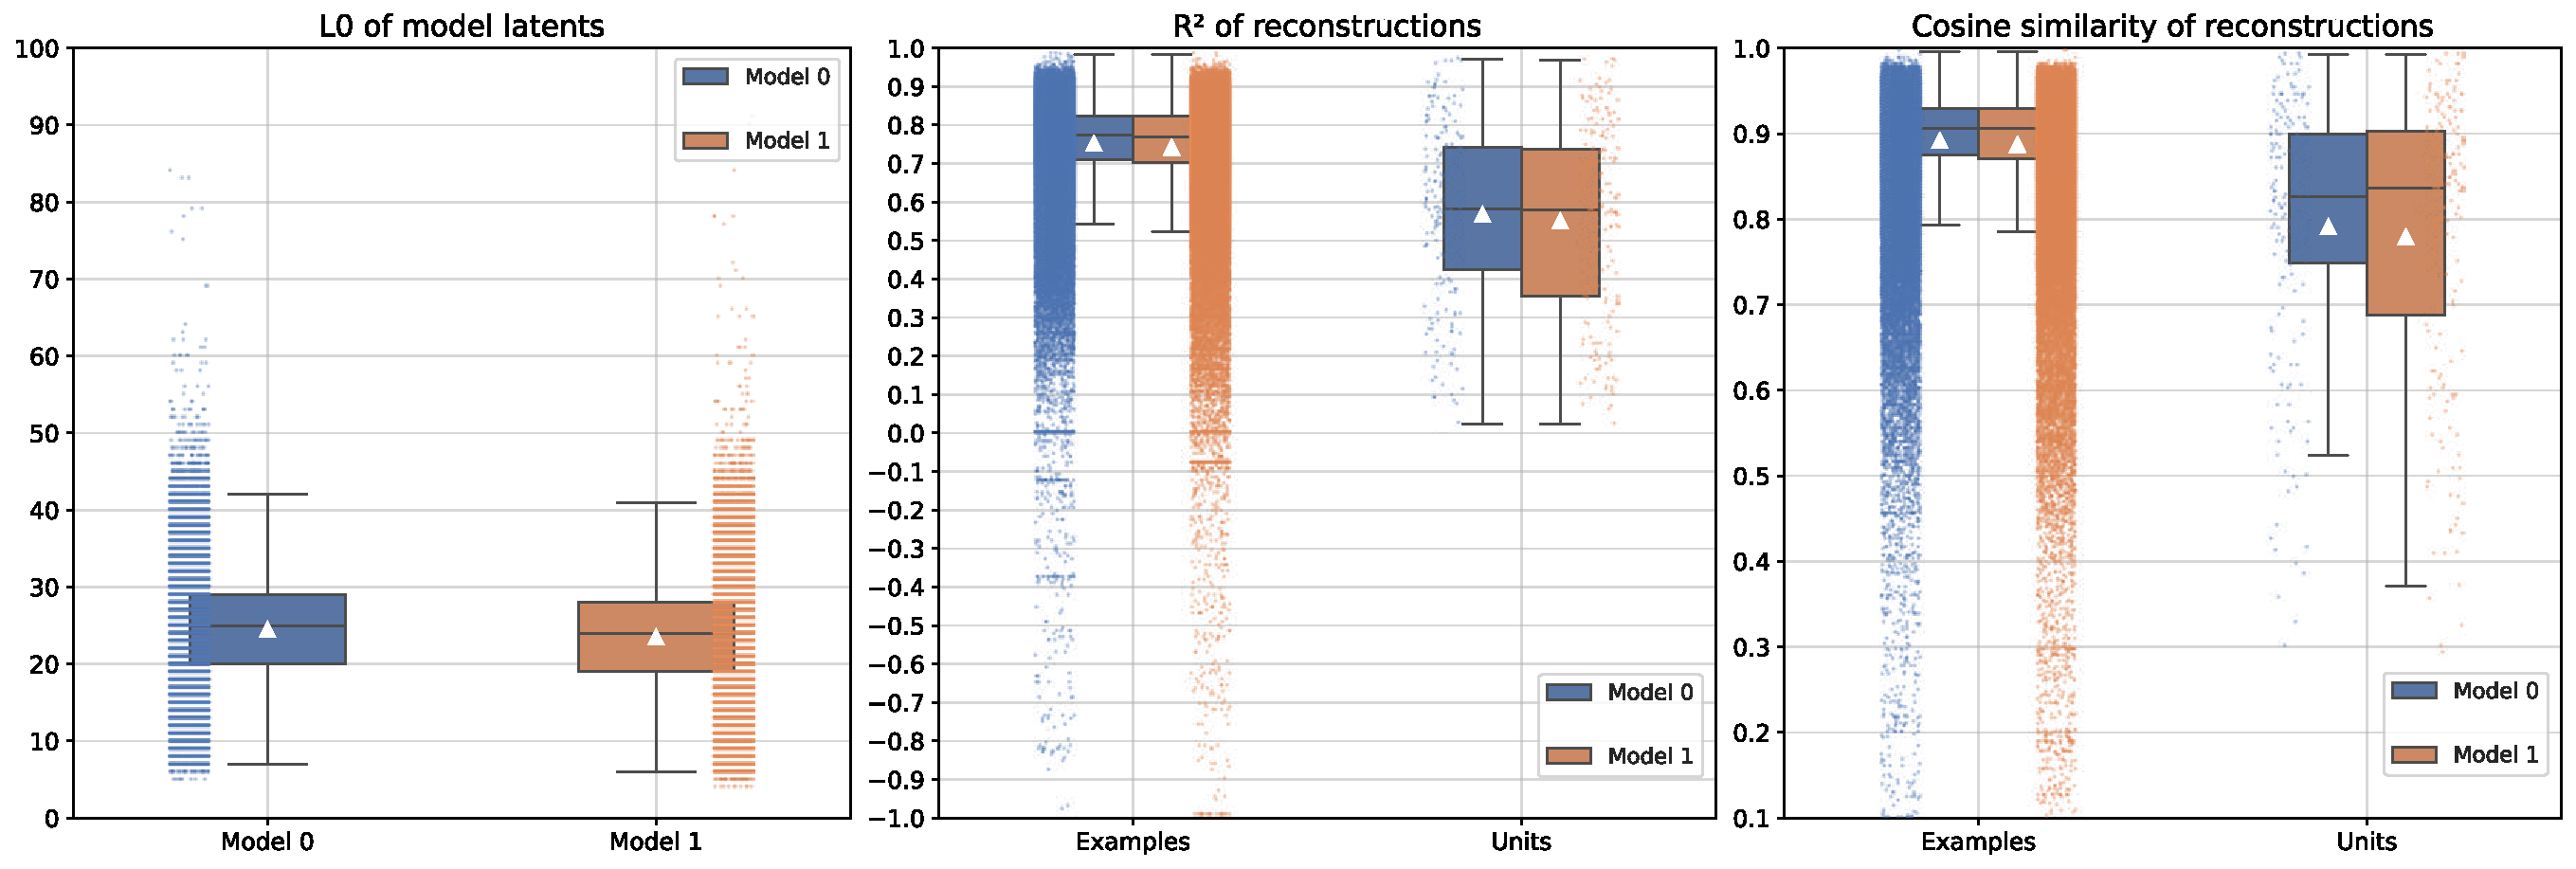
\includegraphics[width=\linewidth]{figures/model_eval.pdf}
    \caption{
        \textbf{Model evaluation metrics.} \\
        \small By default, trained models are evaluated via the following metrics: latent L0 (left), and R\textsuperscript{2} (middle) and cosine similarity (right) of reconstruction-to-actual neural activity for each temporal ("Examples") and spatial ("Units") bin. ... Additional features, such as the R\textsuperscript{2}of overall neural data reconstruction for each individual latent, can be specifed and included.
    }
    \label{figure:model_eval}
\end{figure}

\subsubsection{Hyperparameter sweeps}
\label{subsubsection:hyperparameter_sweeps}

 We typically sweep over key architectural parameters, including the number and size of Matryoshka levels, the batch top-$k$ sparsity coefficient, and the latent space sequence length for the self-attention layer. Additionally, we sweep over optimizer-specific hyperparameters. We use the Adam optimizer by default due to its robust performance across a wide range of deep learning tasks, and typically include its learning rate in the sweep.

 While hyperparameter sweeps are an empirical science, we typically choose these heuristics for setting sweep ranges:

 ...
